\documentclass[journal,12pt,twocolumn]{IEEEtran}
\IEEEoverridecommandlockouts
\usepackage{cite}
\usepackage{amsmath,amssymb,amsfonts,bm}
\usepackage{wasysym}
\usepackage{mathtools}
\usepackage{tkz-euclide} 
\usepackage{tikz}
\usetikzlibrary{calc,math}
 \usepackage{caption}
\usepackage{listings}
\usepackage{gensymb}
\usepackage{enumitem}
\let\vec\mathbf
\numberwithin{equation}{subsection}

\newcommand{\myvec}[1]{\ensuremath{\begin{pmatrix}#1\end{pmatrix}}}
\newcommand{\norm}[1]{\left\lVert#1\right\rVert}
\newcommand{\mydet}[1]{\ensuremath{\begin{vmatrix}#1\end{vmatrix}}}

\renewcommand\thesection{\arabic{section}}
\renewcommand\thesubsection{\thesection.\arabic{subsection}}
\renewcommand\thesubsubsection{\thesubsection.\arabic{subsubsection}}

\renewcommand\thesectiondis{\arabic{section}}
\renewcommand\thesubsectiondis{\thesectiondis.\arabic{subsection}}
\renewcommand\thesubsubsectiondis{\thesubsectiondis.\arabic{subsubsection}}
%\renewcommand{\theequation}{\theenumi}
%\numberwithin{equation}{enumi}

\providecommand{\mbf}{\mathbf}
\providecommand{\pr}[1]{\ensuremath{\Pr\left(#1\right)}}
\providecommand{\qfunc}[1]{\ensuremath{Q\left(#1\right)}}
\providecommand{\sbrak}[1]{\ensuremath{{}\left[#1\right]}}
\providecommand{\lsbrak}[1]{\ensuremath{{}\left[#1\right.}}
\providecommand{\rsbrak}[1]{\ensuremath{{}\left.#1\right]}}
\providecommand{\brak}[1]{\ensuremath{\left(#1\right)}}
\providecommand{\lbrak}[1]{\ensuremath{\left(#1\right.}}
\providecommand{\rbrak}[1]{\ensuremath{\left.#1\right)}}
\providecommand{\cbrak}[1]{\ensuremath{\left\{#1\right\}}}
\providecommand{\lcbrak}[1]{\ensuremath{\left\{#1\right.}}
\providecommand{\rcbrak}[1]{\ensuremath{\left.#1\right\}}}

\lstset{
frame=single, 
breaklines=true,
columns=fullflexible
}

\begin{document}

\title{Matrix Theory EE5609 - Assignment 7\\
}

\author{\IEEEauthorblockN{Sandhya Addetla}\\
\IEEEauthorblockA{PhD Artificial Inteligence Department} \\
AI20RESCH14001\\
 }

\maketitle
\begin{abstract}
Find foot of the perpendicular using SVD
\end{abstract}
Download  python code from 
\begin{lstlisting}
https://github.com/SANDHYA-A/Assignment7
\end{lstlisting}
\section{Problem}
Find the foot of the perpendicular for a point on the line of intersection of planes $9x^2 -4y^2 +z^2 -6xz -4y -1 =0$ on to the plane containing the point $(-1, -4 , 3)$.

\section{Solution}
Given the equation of two intersecting planes is 
\begin{align}
   9x^2 -4y^2 +z^2 -6xz -4y -1 =0\label{2.1}
\end{align}
\begin{enumerate}
\item \textbf{Second order equation in terms of matrices:}\\
The general equation of a second order algebraic surface is given by
\begin{multline}
ax^2 + by^2 + cz^2 + 2dxy + 2exz \\+ 2fyz + 2lx + 2my + 2nz + q = 0.
\end{multline}
This equation can be written as:-
\begin{align}
\vec{x}^T\vec{V}\vec{x} +2 \vec{u}^T\vec{x}+f=0 \label{2.7}\\
\vec{V} = \myvec{a&d&e\\d&b&f\\e&f&c}\quad
\vec{u}= \myvec{l\\m\\n}
\end{align}
Substituting values from the given equation \eqref{2.1}, we get,
\begin{align}
\vec{x}^T\myvec{9&0&-6\\0&-4&0\\-6&0&1}\vec{x} + 2\myvec{0\\-2\\0}^T\vec{x}-1=0
\end{align}
\begin{align}
\vec{V} = \myvec{9&0&-6\\0&-4&0\\-6&0&1} \quad
\vec{u}= \myvec{0\\-2\\0} \quad f=-1
\end{align}
\begin{enumerate}
\item The eigen values of matrix $\vec{V}$ can be calculated as:-
\begin{align}
\mydet{\vec{V} - \lambda\vec{I}} = 0\\
\begin{vmatrix}9-\lambda&0&-6\\0&-4-\lambda&0\\-6&0&1-\lambda\end{vmatrix} = 0\\
\implies -\lambda^3 + 6\lambda^2 + 67\lambda + 108 =0 \\
(-\lambda-4).(\lambda^2 -10\lambda -27) = 0
\end{align}
From above, we get,
\begin{align}
\lambda_1 = -4\\
\lambda_2=-2\sqrt{13} + 5\\
\lambda_3=2\sqrt{13} + 5
\end{align}
The corresponding eigen vectors for these eigen values are:-
\begin{align}
\text{for } \lambda_1 = -4 ,\vec{ v_1} = \myvec{0\\1\\0}
\end{align}
\begin{align}
\text{for } \lambda_2=-2\sqrt{13} + 5 , \vec{ v_2}= \myvec{\frac{\sqrt{13} -2}{3}\\0\\1}\\
\text{for } \lambda_3=2\sqrt{13} + 5 , \vec{ v_3} = \myvec{\frac{-\sqrt{13} -2}{3}\\0\\1}
\end{align}
Eigen vectors matrix is
\begin{align}
\myvec{0 &\frac{\sqrt{13} -2}{3}&-\frac{\sqrt{13} -2}{3}\\1 &0&0\\0&1&1}
\end{align}
The normalizing these values, we obtain
\begin{align}
\myvec{0 &\frac{\sqrt{13} -2}{\sqrt{26-4\sqrt{13}}}&\frac{-\sqrt{13} -2}{\sqrt{26+4\sqrt{13}}}\\1 &0&0\\0&\frac{3}{\sqrt{26-4\sqrt{13}}}&\frac{3}{\sqrt{26+4\sqrt{13}}}}
\end{align}
\item Affine transformation:\\
We can obtain the affine transformation for equation at \eqref{2.7} by taking the value of $\vec{x}$ as:
\begin{align}
\vec{x} = \vec{P}\vec{y} + c   \label{2.19.1}
\end{align}
such that
\begin{align}
\vec{P}^T\vec{V}\vec{P}= \vec{D} \\ 
\vec{D}=\myvec{\lambda_1&0&0\\0&\lambda_2&0\\0&0&\lambda_3}
\end{align}
and $\vec{P}$ is the transformation matrix and can be given by the normalized eigen vectors of matrix $\vec{V}$. Therefore,
\begin{align}
\vec{P} = \myvec{0 &\frac{\sqrt{13} -2}{\sqrt{26-4\sqrt{13}}}&\frac{-\sqrt{13} -2}{\sqrt{26+4\sqrt{13}}}\\1 &0&0\\0&\frac{3}{\sqrt{26-4\sqrt{13}}}&\frac{3}{\sqrt{26+4\sqrt{13}}}}
\end{align}
Also, $\vec{P}^T = \vec{P}^{-1}$

\begin{multline}
\vec{P}^T\vec{V}\vec{P}= \myvec{0&1&0\\
\frac{\sqrt{13} -2}{\sqrt{26-4\sqrt{13}}}&0&\frac{3}{\sqrt{26-4\sqrt{13}}}\\
\frac{-\sqrt{13} -2}{\sqrt{26+4\sqrt{13}}}&0&\frac{3}{\sqrt{26+4\sqrt{13}}}
}  \\ \myvec{9&0&-6\\0&-4&0\\-6&0&1}   
\myvec{0 &\frac{\sqrt{13} -2}{\sqrt{26-4\sqrt{13}}}&\frac{-\sqrt{13} -2}{\sqrt{26+4\sqrt{13}}}\\1 &0&0\\0&\frac{3}{\sqrt{26-4\sqrt{13}}}&\frac{3}{\sqrt{26+4\sqrt{13}}}}
\end{multline}
\begin{align}
=\myvec{-4&0&0\\0&-2\sqrt{13}+5&0\\0&0&2\sqrt{13}+5} = \vec{D}
\end{align}
 \eqref{2.7}  can be expressed as:
\begin{align}
\vec{y}^T\vec{D}\vec{y} = \vec{u}^T\vec{V}^{-1}\vec{u} -f   \quad     \wasytherefore |\vec{V}| \neq 0
\end{align}
\begin{multline}
\vec{u}^T\vec{V}^{-1}\vec{u} \\= \myvec{0&-2&0} \myvec{\frac{-1}{27} & 0 &\frac{-2}{9}\\ 0 & \frac{-1}{4} & 0 \\ \frac{-2}{9} & 0 &\frac{-1}{3}}\myvec{0\\-2\\0}\\=-1
\end{multline}
Therefore, we obtain
\begin{align}
\vec{y}^T\myvec{-4&0&0\\0&-2\sqrt{13}+5&0\\0&0&2\sqrt{13}+5}\vec{y} = 0  \label{2.27.1}
\end{align}
\begin{figure}[h]
    \centering
    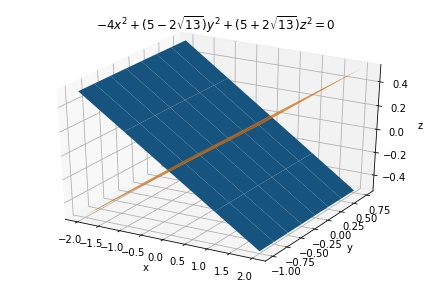
\includegraphics[width=\columnwidth]{planes.jpg}
    \caption{Plot of intersecting planes}
    \label{Fig :1}
\end{figure}
\item Obtaining equation of planes from transformation\\
From \eqref{2.19.1} we can write $\vec{y}$ as
\begin{align}
\vec{y} = \vec{P}^{-1}(\vec{x} - c)
\end{align}
\begin{align}
\vec{y} =  \myvec{0&1&0\\
\frac{\sqrt{13} -2}{\sqrt{26-4\sqrt{13}}}&0&\frac{3}{\sqrt{26-4\sqrt{13}}}\\
\frac{-\sqrt{13} -2}{\sqrt{26+4\sqrt{13}}}&0&\frac{3}{\sqrt{26+4\sqrt{13}}}
} \myvec{x-0\\y-1/2\\z-0}
\end{align}
\begin{align}
\vec{y} = \myvec{y-\frac{1}{2}\\ \frac{(\sqrt{13} -2)x +3z}{26-4\sqrt{13}}\\\frac{(-\sqrt{13} -2)x +3z}{26+4\sqrt{13}}}
\end{align}
Substituting value of $\vec{y}$ in \eqref{2.27.1}, we obtain:
\begin{multline}
\myvec{y-\frac{1}{2}&\frac{(\sqrt{13} -2)x +3z}{26-4\sqrt{13}}&\frac{(-\sqrt{13} -2)x +3z}{26+4\sqrt{13}}}\\
\myvec{-4&0&0\\0&-2\sqrt{13}+5&0\\0&0&2\sqrt{13}+5}\\ \myvec{y-\frac{1}{2}\\ \frac{(\sqrt{13} -2)x +3z}{26-4\sqrt{13}}\\\frac{(-\sqrt{13} -2)x +3z}{26+4\sqrt{13}}} = 0
\end{multline}
\begin{align}
\implies   9x^2 -4y^2 +z^2 -6xz -4y -1 =0
\end{align}
Expressing in terms of individual plane equations, we get
\begin{align}
   ( 3x- 2y -z -1)( 3x +2y-z +1 ) = 0 
\end{align}
\end{enumerate}

\item \textbf{Finding equation of individual planes:}\\
Let the two normals for these planes be $\vec{n_1}$ and $\vec{n_2}$
\begin{align}
   a_{1}x+ b_{1}y +c_{1}z +d_{1} =0\label{2.2}\\
  a_{2}x +b_{2}y +c_{2}z +d_{2} =0\label{2.3}
\end{align}
We have,
\begin{align}
   (  a_{1}x+ b_{1}y +c_{1}z +d_{1})( a_{2}x +b_{2}y +c_{2}z +d_{2} ) = 0 \label{2.5}
\end{align}
From equation \eqref{2.1} and \eqref{2.5} we get the equations of two planes as:
\begin{align}
   ( 3x- 2y -z -1)( 3x +2y-z +1 ) = 0 \label{2.6}\\
   3x- 2y -z -1 = 0  \label{2.10} \\
 3x +2y-z +1  = 0 \label{2.11}
\end{align}
\item \textbf{Equation of normal to individual planes:}\\
Let equation \eqref {2.10} and \eqref{2.11} be denoted as $E_{1 }$ and $ E_{2}$. Let $ k_{1}$ and $k_{2}$ be two arbitrary constants. Then,
 \begin{align}
   k_{1}E_{1} + k_{2}E_{2} = 0\label{2.8}
\end{align}
represents a linear equation and this equation will be satisifed by coordinates of the points that lie on both these planes.\\
 Let us assume the constants $ k_{1} = 1$  and $k_{2} = 1$.\\
Then the resultant equation from \eqref{2.8} represents a plane through the line of intersection of the planes $E_{1}$ and $E_{2}$ and is given by:
\begin{multline}
   1.(3x- 2y -z -1) + \\1.( 3x +2y-z +1 ) =0
\end{multline}
\begin{align}
  3x = z\\ 
\myvec{3& 0& -1} \vec{x} = 0   \label{2.9}
\end{align}
\item \textbf{Equation of line of intersection of planes:}\\
Equation \eqref {2.9} is the equation of the normal to  $E_{1}$ and $E_{2}$. Also, from equation \eqref{2.10} and     \eqref {2.11}, we obtain the equation of line of intersection of the given planes  as
\begin{align}
   3x = z \text{ and } y =\frac{-1}{2}\label{2.16}
\end{align}
\item \textbf{Equation of plane passing through point (-1, -4 ,3) and perpendicular to plane at \eqref{2.9}:}\\

Let, $\vec{r}$ be \myvec{x& y& z}. Now, the equation of the plane passing through the point Q(-1, -4 ,3) can be obtained by
\begin{align}
    \vec{n} . ( \vec{r} - \vec{Q}) = 0  \label{2.12}\\
    \myvec{3 & 0 & -1} \myvec{x+1 \\ y+4 \\ z-3} = 0
\end{align}
Thus, equation of the plane containing the point$(-1, -4 , 3)$ is obtained as
\begin{align}
    \myvec{3 & 0 & -1} \vec{x} = -6 \label{2.14}
\end{align}
\item \textbf{Finding normal vectors:}\\
The equation of the plane at \eqref{2.14} can be expressed as:
\begin{align}\label{eq1}
	\vec{n}^T\vec{x} &= c
\end{align}
Rewriting given equation of plane in \eqref{eq1} form
\begin{align}\label{eq2}
	\myvec{3 & 0 & -1}\myvec{x\\y\\z} &= -6
\end{align}
where the value of 
\begin{align}
    \vec{n} &= \myvec{3\\0\\-1} \\
    \vec{x} &= \myvec{x\\y\\z} \\
    c &= -6
\end{align}
The two vectors $\vec{q}$ and $\vec{r}$ which are $\perp$ to $\vec{n}$ can be obtained by 
\begin{align}
	\myvec{3 & 0 & -1}\myvec{a\\b\\c} = 0\\
	\implies 3a - c = 0 \label{eq4}
\end{align}
Put $a=0$ and $b=1$ in \eqref{eq4}, $\implies c=0$\\
Put $a=1$ and $b=0$ in \eqref{eq4}, $\implies c=3$\\

Hence 
\begin{align}
\vec{q} = \myvec{0\\1\\0}, \vec{r} = \myvec{1\\0\\3}
\end{align}
An arbitrary point on line of intersection of two planes at equation \eqref{2.1} can be taken as:
\begin{equation}
	\vec{b} = \myvec{1 \\ \frac{-1}{2} \\ 3} \label{2.28}
\end{equation}
\item \textbf{Solution using Singular Value Decomposition:}\\
So, now we have two orthogonal vectors $\vec{q}$ and $\vec{r}$ and $\vec{M}$ is the matrix of these orthogonal vectors. We  can solve the equation :
\begin{align}
\vec{M}\vec{x} &= \vec{b}\label{eq11} 
\end{align}
Substituting the values of normal vectors and the point on the plane in \eqref{eq11} , we get,
\begin{align}
 \myvec{0 &1\\1 & 0\\0 & 3} \vec{x} = 	 \myvec{1 \\ \frac{-1}{2} \\ 3}
 \end{align}

To solve the above equation, we  perform Singular Value Decomposition on $\vec{M}$ as follows,
\begin{align}
\vec{M}=\vec{U}\vec{S}\vec{V}^T \label{2.20}
\end{align}

Where the columns of $\vec{V}$ are the eigen vectors of $\vec{M}^T\vec{M}$ ,the columns of $\vec{U}$ are the eigen vectors of $\vec{M}\vec{M}^T$ and $\vec{S}$ is diagonal matrix of singular value of eigenvalues of $\vec{M}^T\vec{M}$.
\begin{align}
    \vec{M}^T\vec{M} &= \myvec{1 & 0\\0 & 10} \\
    \vec{M}\vec{M}^T &= \myvec{1 & 0& 3\\0 & 1 & 0\\ 3 & 0 & 9} 
\end{align}
As we know that,
\begin{align}
    \vec{U} \vec{S} \vec{V}^T \vec{x} = \vec{b} \nonumber \\
    \implies \vec{x} = \vec{V} \vec{S_+} \vec{U^T} \vec{b} \label{eq:eq_9}
\end{align}
Where $\vec{S_+}$ is Moore-Penrose Pseudo-Inverse of $\vec{S}$.
\begin{enumerate}
\item \textbf{Calculating eigenvalues and eigen vectors of $\vec{M}\vec{M}^T$: }
\begin{align}
    \mydet{\vec{M} \vec{M}^T - \lambda \vec{I}} = 0 \nonumber \\
    \implies \mydet{1-\lambda & 0& 3\\0 & 1-\lambda & 0\\ 3 & 0 & 9-\lambda} &= 0 \nonumber \\
    \implies -\lambda^3 +11\lambda^2 -10\lambda =0 \nonumber
\end{align}
Hence eigenvalues of $\vec{M}\vec{M}^T$ are,
\begin{align} \label{eq:eq_10}
    \lambda_1 = 10; \quad \lambda_2 = 1; \quad \lambda_3 =0
\end{align}
And the corresponding eigenvectors are,
\begin{align}
    \vec{u_1} = \myvec{\frac{1}{3} \\ 0 \\ 1}; \quad \vec{u_2} = \myvec{0 \\ 1 \\ 0}; \quad
    \vec{u_3} = \myvec{-3\\ 0 \\ 1} \label{eq:eq_11} 
\end{align}
Normalizing the eigen vectors we get,
\begin{align}
\vec{u}_1=\myvec{\frac{1}{\sqrt{10}}\\0\\\frac{3}{\sqrt{10}}},
\vec{u}_2=\myvec{0\\1\\0},
\vec{u}_3=\myvec{-\frac{3}{\sqrt{10}}\\0\\\frac{1}{\sqrt{10}}}
\end{align}
$\vec{U}$ is obtained as  follows,
\begin{align}
 \vec{U}=  \myvec{\frac{1}{\sqrt{10}}& 0&-\frac{3}{\sqrt{10}}\\
0&1&0\\
\frac{3}{\sqrt{10}}&0&\frac{1}{\sqrt{10}}}  \label{2.30}
\end{align}
Using values from \eqref{eq:eq_10},
\begin{align} \label{eq:eq_14}
    \vec{S} = \myvec{\sqrt{10} & 0 \\ 0 & 1 \\ 0 & 0} 
\end{align}
\item \textbf{Calculating eigen values and eigen vectors of  $\vec{M}^T\vec{M}$:}
\begin{align}
    \mydet{\vec{M}^T\vec{M} - \lambda \vec{I}} = 0 \nonumber \\
    \implies \mydet{1-\lambda & 0 \\ 0 & 10-\lambda} &= 0 \nonumber \\
    \implies \lambda^2 -11\lambda + 10 &= 0 \nonumber
\end{align}
Hence, eigenvalues of $\vec{M}^T\vec{M}$ are,
\begin{align}
    \lambda_4 =10; \quad \lambda_5 = 1 \nonumber
\end{align}
And the corresponding eigenvectors are,
\begin{align}
    \vec{v}_1 = \myvec{0 \\ 1}; \quad 
    \vec{v}_2 =  \myvec{1 \\ 0}\label{eq:eq_15}
\end{align}
From \eqref{eq:eq_15} we obtain $\vec{V}$ as,
\begin{align} \label{eq:eq_16}
    \vec{V} = \myvec{0 & 1 \\ 1 & 0}
\end{align}
Hence we obtain SVD of $\vec{M}$ as :
\begin{align}
	\vec{M}  =  \myvec{\frac{1}{\sqrt{10}}& 0&-\frac{3}{\sqrt{10}}\\
0&1&0\\ \frac{3}{\sqrt{10}}&0&\frac{1}{\sqrt{10}}}\myvec{\sqrt{10} & 0 \\ 0 & 1 \\ 0 & 0} \myvec{0 & 1 \\ 1 & 0}
\end{align}
Moore-Penrose Pseudo inverse of $\vec{S}$ is obtained as,
\begin{align}
\vec{S_+} = \myvec{\frac{1}{\sqrt{10}}&0&0\\0&1&0}  \label{2.41}
\end{align}
Using equation \eqref{2.28},\eqref{2.30}, \eqref{eq:eq_16} and \eqref{2.41} in equation \eqref{eq:eq_9} we obtain value of $\vec{x}$ as:
\begin{align}
\vec{U}^T\vec{b}=\myvec{\sqrt{10} \\ \frac{-1}{2}\\ 0}\\
\vec{S_+}\vec{U}^T\vec{b}=\myvec{1\\ \frac{-1}{2}}\\
\vec{x} = \vec{V}\vec{S_+}\vec{U}^T\vec{b} = \myvec{\frac{-1}{2}\\1} \label{2.44}
\end{align}
\end{enumerate}
\item \textbf{Solution verification:}\\
We can verify the obtained solution,
\begin{align}
\vec{M}^T\vec{M}\vec{x} = \vec{M}^T\vec{b} \label{2.45}
\end{align}
Computing the RHS values in equation \ref{2.45}, we get,
\begin{align}
\vec{M}^T\vec{M}\vec{x} &= \myvec{\frac{-1}{2}\\10}\\
\implies\myvec{1&0\\0&10}\vec{x} &= \myvec{\frac{-1}{2}\\10} \label{eq2.47}
\end{align}
The values of $\vec{x}$ is obtained as:
\begin{align}
\vec{x} &= \myvec{\frac{-1}{2}\\1} \label{2.70}
\end{align}
Comparing equation \eqref{2.44} and \eqref{2.70} solution is verified.

\end{enumerate}


\end{document}
